\documentclass{standalone}
\usepackage{tikz}
\usepackage{xcolor}
\usetikzlibrary{patterns, positioning}
\usetikzlibrary{shapes.misc}
\usepackage[outline]{contour}
\contourlength{1.5pt} 


\begin{document}
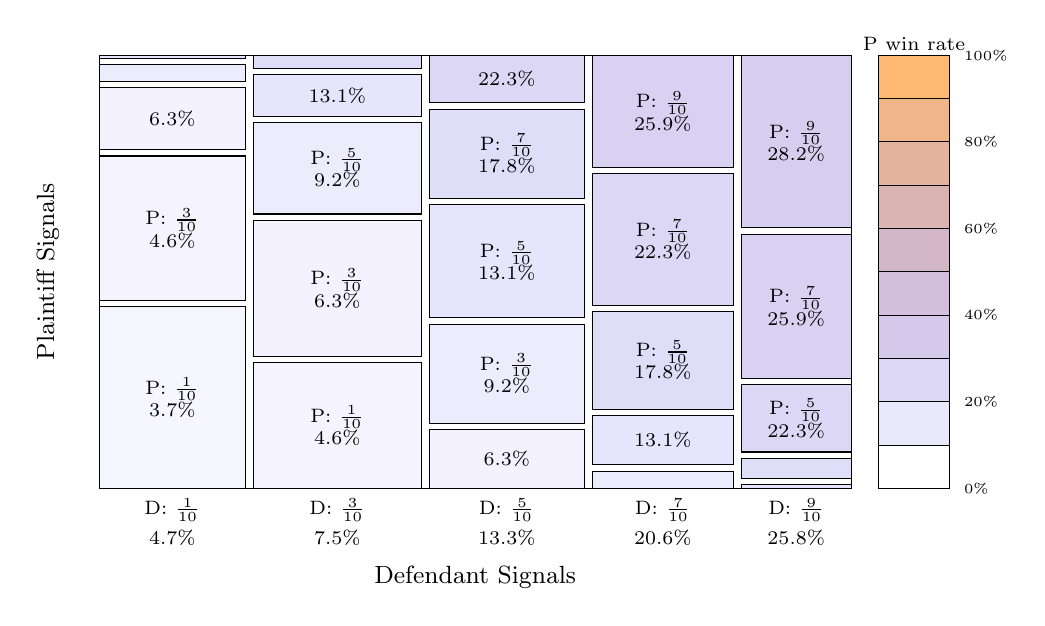
\begin{tikzpicture}
\newcommand{\DFractionOffset}{0.4}
\newcommand{\AxisLabelYAdjust}{-0.235}
\draw[draw=black] (0.6,2) rectangle (10.15,7.5);
\draw[fill=blue!96!orange!4!white!87!white, draw=black] (0.6,2) rectangle (2.4578,4.3056);
\draw (1.5289049386578777, 3.1527772129595677) node[font=\scriptsize, text=black, align=center] {P: $\frac{1}{10}$\\ 3.7\%};
\draw[fill=blue!95!orange!5!white!86!white, draw=black] (0.6,4.3856) rectangle (2.4578,6.2207);
\draw (1.5289049386578777, 5.303109912388211) node[font=\scriptsize, text=black, align=center] {P: $\frac{3}{10}$\\ 4.6\%};
\draw[fill=blue!94!orange!6!white!86!white, draw=black] (0.6,6.3007) rectangle (2.4578,7.0911);
\draw (1.5289049386578777, 6.695893657892247) node[font=\scriptsize, text=black, align=center] {6.3\%};
\draw[fill=blue!91!orange!9!white!85!white, draw=black] (0.6,7.1711) rectangle (2.4578,7.3821);
\draw[fill=blue!87!orange!13!white!84!white, draw=black] (0.6,7.4621) rectangle (2.4578,7.5);
\draw (1.5289049386578777, 1.6) node[anchor=north, font=\scriptsize, text=black] {4.7\%};
\draw (1.5289049386578777, {1.6 + \DFractionOffset}) node[anchor=north, font=\scriptsize, text=black] {D: $\frac{1}{10}$};
\draw[fill=blue!95!orange!5!white!86!white, draw=black] (2.5578,2) rectangle (4.6935,3.5964);
\draw (3.6256320501499077, 2.798187043271046) node[font=\scriptsize, text=black, align=center] {P: $\frac{1}{10}$\\ 4.6\%};
\draw[fill=blue!94!orange!6!white!86!white, draw=black] (2.5578,3.6764) rectangle (4.6935,5.4053);
\draw (3.6256320501499077, 4.540833799449219) node[font=\scriptsize, text=black, align=center] {P: $\frac{3}{10}$\\ 6.3\%};
\draw[fill=blue!91!orange!9!white!85!white, draw=black] (2.5578,5.4853) rectangle (4.6935,6.6481);
\draw (3.6256320501499077, 6.066699651365936) node[font=\scriptsize, text=black, align=center] {P: $\frac{5}{10}$\\ 9.2\%};
\draw[fill=blue!87!orange!13!white!84!white, draw=black] (2.5578,6.7281) rectangle (4.6935,7.2555);
\draw (3.6256320501499077, 6.9918032982678735) node[font=\scriptsize, text=black, align=center] {13.1\%};
\draw[fill=blue!82!orange!18!white!82!white, draw=black] (2.5578,7.3355) rectangle (4.6935,7.5);
\draw (3.6256320501499077, 1.6) node[anchor=north, font=\scriptsize, text=black] {7.5\%};
\draw (3.6256320501499077, {1.6 + \DFractionOffset}) node[anchor=north, font=\scriptsize, text=black] {D: $\frac{3}{10}$};
\draw[fill=blue!94!orange!6!white!86!white, draw=black] (4.7935,2) rectangle (6.7625,2.7458);
\draw (5.77795949992813, 2.372907581414198) node[font=\scriptsize, text=black, align=center] {6.3\%};
\draw[fill=blue!91!orange!9!white!85!white, draw=black] (4.7935,2.8258) rectangle (6.7625,4.087);
\draw (5.77795949992813, 3.4564246488267196) node[font=\scriptsize, text=black, align=center] {P: $\frac{3}{10}$\\ 9.2\%};
\draw[fill=blue!87!orange!13!white!84!white, draw=black] (4.7935,4.167) rectangle (6.7625,5.6057);
\draw (5.77795949992813, 4.8863458902017065) node[font=\scriptsize, text=black, align=center] {P: $\frac{5}{10}$\\ 13.1\%};
\draw[fill=blue!82!orange!18!white!82!white, draw=black] (4.7935,5.6857) rectangle (6.7625,6.8159);
\draw (5.77795949992813, 6.2507680933855925) node[font=\scriptsize, text=black, align=center] {P: $\frac{7}{10}$\\ 17.8\%};
\draw[fill=blue!78!orange!22!white!81!white, draw=black] (4.7935,6.8959) rectangle (6.7625,7.5);
\draw (5.77795949992813, 7.1979392705964065) node[font=\scriptsize, text=black, align=center] {22.3\%};
\draw (5.77795949992813, 1.6) node[anchor=north, font=\scriptsize, text=black] {13.3\%};
\draw (5.77795949992813, {1.6 + \DFractionOffset}) node[anchor=north, font=\scriptsize, text=black] {D: $\frac{5}{10}$};
\draw[fill=blue!91!orange!9!white!85!white, draw=black] (6.8625,2) rectangle (8.6558,2.2186);
\draw[fill=blue!87!orange!13!white!84!white, draw=black] (6.8625,2.2986) rectangle (8.6558,2.9266);
\draw (7.759131226979639, 2.612617492906414) node[font=\scriptsize, text=black, align=center] {13.1\%};
\draw[fill=blue!82!orange!18!white!82!white, draw=black] (6.8625,3.0066) rectangle (8.6558,4.2476);
\draw (7.759131226979639, 3.627119128013417) node[font=\scriptsize, text=black, align=center] {P: $\frac{5}{10}$\\ 17.8\%};
\draw[fill=blue!78!orange!22!white!81!white, draw=black] (6.8625,4.3276) rectangle (8.6558,5.9953);
\draw (7.759131226979639, 5.161467588102817) node[font=\scriptsize, text=black, align=center] {P: $\frac{7}{10}$\\ 22.3\%};
\draw[fill=blue!74!orange!26!white!79!white, draw=black] (6.8625,6.0753) rectangle (8.6558,7.5);
\draw (7.759131226979639, 6.787673255160696) node[font=\scriptsize, text=black, align=center] {P: $\frac{9}{10}$\\ 25.9\%};
\draw (7.759131226979639, 1.6) node[anchor=north, font=\scriptsize, text=black] {20.6\%};
\draw (7.759131226979639, {1.6 + \DFractionOffset}) node[anchor=north, font=\scriptsize, text=black] {D: $\frac{7}{10}$};
\draw[fill=blue!87!orange!13!white!84!white, draw=black] (8.7558,2) rectangle (10.15,2.0505);
\draw[fill=blue!82!orange!18!white!82!white, draw=black] (8.7558,2.1305) rectangle (10.15,2.3825);
\draw[fill=blue!78!orange!22!white!81!white, draw=black] (8.7558,2.4625) rectangle (10.15,3.3156);
\draw (9.452898838543536, 2.889050798449539) node[font=\scriptsize, text=black, align=center] {P: $\frac{5}{10}$\\ 22.3\%};
\draw[fill=blue!74!orange!26!white!79!white, draw=black] (8.7558,3.3956) rectangle (10.15,5.2281);
\draw (9.452898838543536, 4.311897328372477) node[font=\scriptsize, text=black, align=center] {P: $\frac{7}{10}$\\ 25.9\%};
\draw[fill=blue!72!orange!28!white!79!white, draw=black] (8.7558,5.3081) rectangle (10.15,7.5);
\draw (9.452898838543536, 6.404074061852454) node[font=\scriptsize, text=black, align=center] {P: $\frac{9}{10}$\\ 28.2\%};
\draw (9.452898838543536, 1.6) node[anchor=north, font=\scriptsize, text=black] {25.8\%};
\draw (9.452898838543536, {1.6 + \DFractionOffset}) node[anchor=north, font=\scriptsize, text=black] {D: $\frac{9}{10}$};
\node[font=\small, text=black] at (5.375, {1.1 + \AxisLabelYAdjust}) {Defendant Signals};
\node[font=\small, text=black, rotate=90] at (-0.050000000000000044, 4.75) {Plaintiff Signals};
\draw[draw=black] (10.5,2) rectangle (11.4,7.5);
\draw (10.95, 7.65) node[font=\scriptsize, text=black] {P win rate};
\draw[fill=blue!100!orange!0!white!88!white, draw=black] (10.5,2) rectangle (11.4,2.55);
\draw[fill=blue!89!orange!11!white!84!white, draw=black] (10.5,2.55) rectangle (11.4,3.1);
\draw[fill=blue!78!orange!22!white!81!white, draw=black] (10.5,3.1) rectangle (11.4,3.65);
\draw[fill=blue!67!orange!33!white!77!white, draw=black] (10.5,3.65) rectangle (11.4,4.2);
\draw[fill=blue!56!orange!44!white!73!white, draw=black] (10.5,4.2) rectangle (11.4,4.75);
\draw[fill=blue!44!orange!56!white!70!white, draw=black] (10.5,4.75) rectangle (11.4,5.3);
\draw[fill=blue!33!orange!67!white!66!white, draw=black] (10.5,5.3) rectangle (11.4,5.85);
\draw[fill=blue!22!orange!78!white!62!white, draw=black] (10.5,5.85) rectangle (11.4,6.4);
\draw[fill=blue!11!orange!89!white!59!white, draw=black] (10.5,6.4) rectangle (11.4,6.95);
\draw[fill=blue!0!orange!100!white!55!white, draw=black] (10.5,6.95) rectangle (11.4,7.5);
\draw (11.46, 2) node[anchor=west, font=\tiny, text=black] {0\%};
\draw (11.46, 3.1) node[anchor=west, font=\tiny, text=black] {20\%};
\draw (11.46, 4.2) node[anchor=west, font=\tiny, text=black] {40\%};
\draw (11.46, 5.3) node[anchor=west, font=\tiny, text=black] {60\%};
\draw (11.46, 6.4) node[anchor=west, font=\tiny, text=black] {80\%};
\draw (11.46, 7.5) node[anchor=west, font=\tiny, text=black] {100\%};


\end{tikzpicture}
\end{document}